%! Author = elias
%! Date = 2/5/23

% Preamble
\documentclass{beamer}

% Packages
\usepackage{amsmath}
\usepackage[utf8]{inputenc}
\usepackage{blkarray}
\usepackage{pgfplots}
\usepackage{tikz}
\usepackage{siunitx}
\usepackage{color}
\usepackage{graphicx}

\usepgfplotslibrary{units} % Allows to enter the units nicely
\pgfplotsset{compat=1.18}

\usetheme{Madrid}
\usecolortheme{beaver}

\title {Ball fangender Roboterarm}
\date[Maturaarbeit]{}

\subtitle{Maturaarbeit 2023}

\author{Elias Bauer}
\institute{Kollegium St. Fidelis}

\beamertemplatenavigationsymbolsempty

% Document
\begin{document}



    \frame[plain]{\titlepage}


    \begin{frame}
        \frametitle{Flugbahn - X Achse}

        \begin{tikzpicture}
            \begin{axis} [
                xmin = 0, xmax = 0.7,
                ymin = -3, ymax= 3,
                grid=major, % Display a grid
                grid style={dashed, red!30},
                xlabel=Zeit,
                ylabel=Position,
                x unit=\si{\second}, % Set the respective units
                y unit=\si{\meter},
            ]

                \addplot[
                    domain = 0:0.7,
                    smooth,
                    ultra thick,
                    gray!50
                ] {2.626712480 * x + -2.005835704};

                \addplot[
                    domain = 0:0.7,
                    smooth,
                    only marks,
                    red,
                ] file[skip first] {FlightPathX.dat};


            \end{axis}
        \end{tikzpicture}

    \end{frame}

    \begin{frame}
        \frametitle{Flugbahn - Y Achse}

        \begin{tikzpicture}
            \begin{axis} [
                xmin = 0, xmax = 0.7,
                ymin = -3, ymax = 3,
                grid=major, % Display a grid
                grid style={dashed, green!30},
                xlabel=Zeit,
                ylabel=Position,
                x unit=\si{\second}, % Set the respective units
                y unit=\si{\meter},
            ]

                \addplot[
                    domain = 0:0.7,
                    smooth,
                    ultra thick,
                    gray!50
                ] {-0.019158488 * x + 0.029724438};

                \addplot[
                    domain = 0:0.7,
                    smooth,
                    only marks,
                    green,
                ] file[skip first] {FlightPathY.dat};


            \end{axis}
        \end{tikzpicture}

    \end{frame}

    \begin{frame}
        \frametitle{Flugbahn - Höhe}

        \begin{tikzpicture}
            \begin{axis} [
                xmin = 0, xmax = 0.7,
                grid=major, % Display a grid
                grid style={dashed, blue!30},
                xlabel=Zeit,
                ylabel=Höhe,
                x unit=\si{\second}, % Set the respective units
                y unit=\si{\meter},
            ]

                \addplot[
                    domain = 0:0.7,
                    smooth,
                    ultra thick,
                    gray!50
                ] {-5.170016538 * x * x + 3.026370508 * x + 0.539997655};

                \addplot[
                    domain = 0:0.7,
                    smooth,
                    only marks,
                    blue,
                ] file[skip first] {FlightPathZ.dat};


            \end{axis}
        \end{tikzpicture}

    \end{frame}

    \begin{frame}
        \frametitle{Bauspezifikationen}
        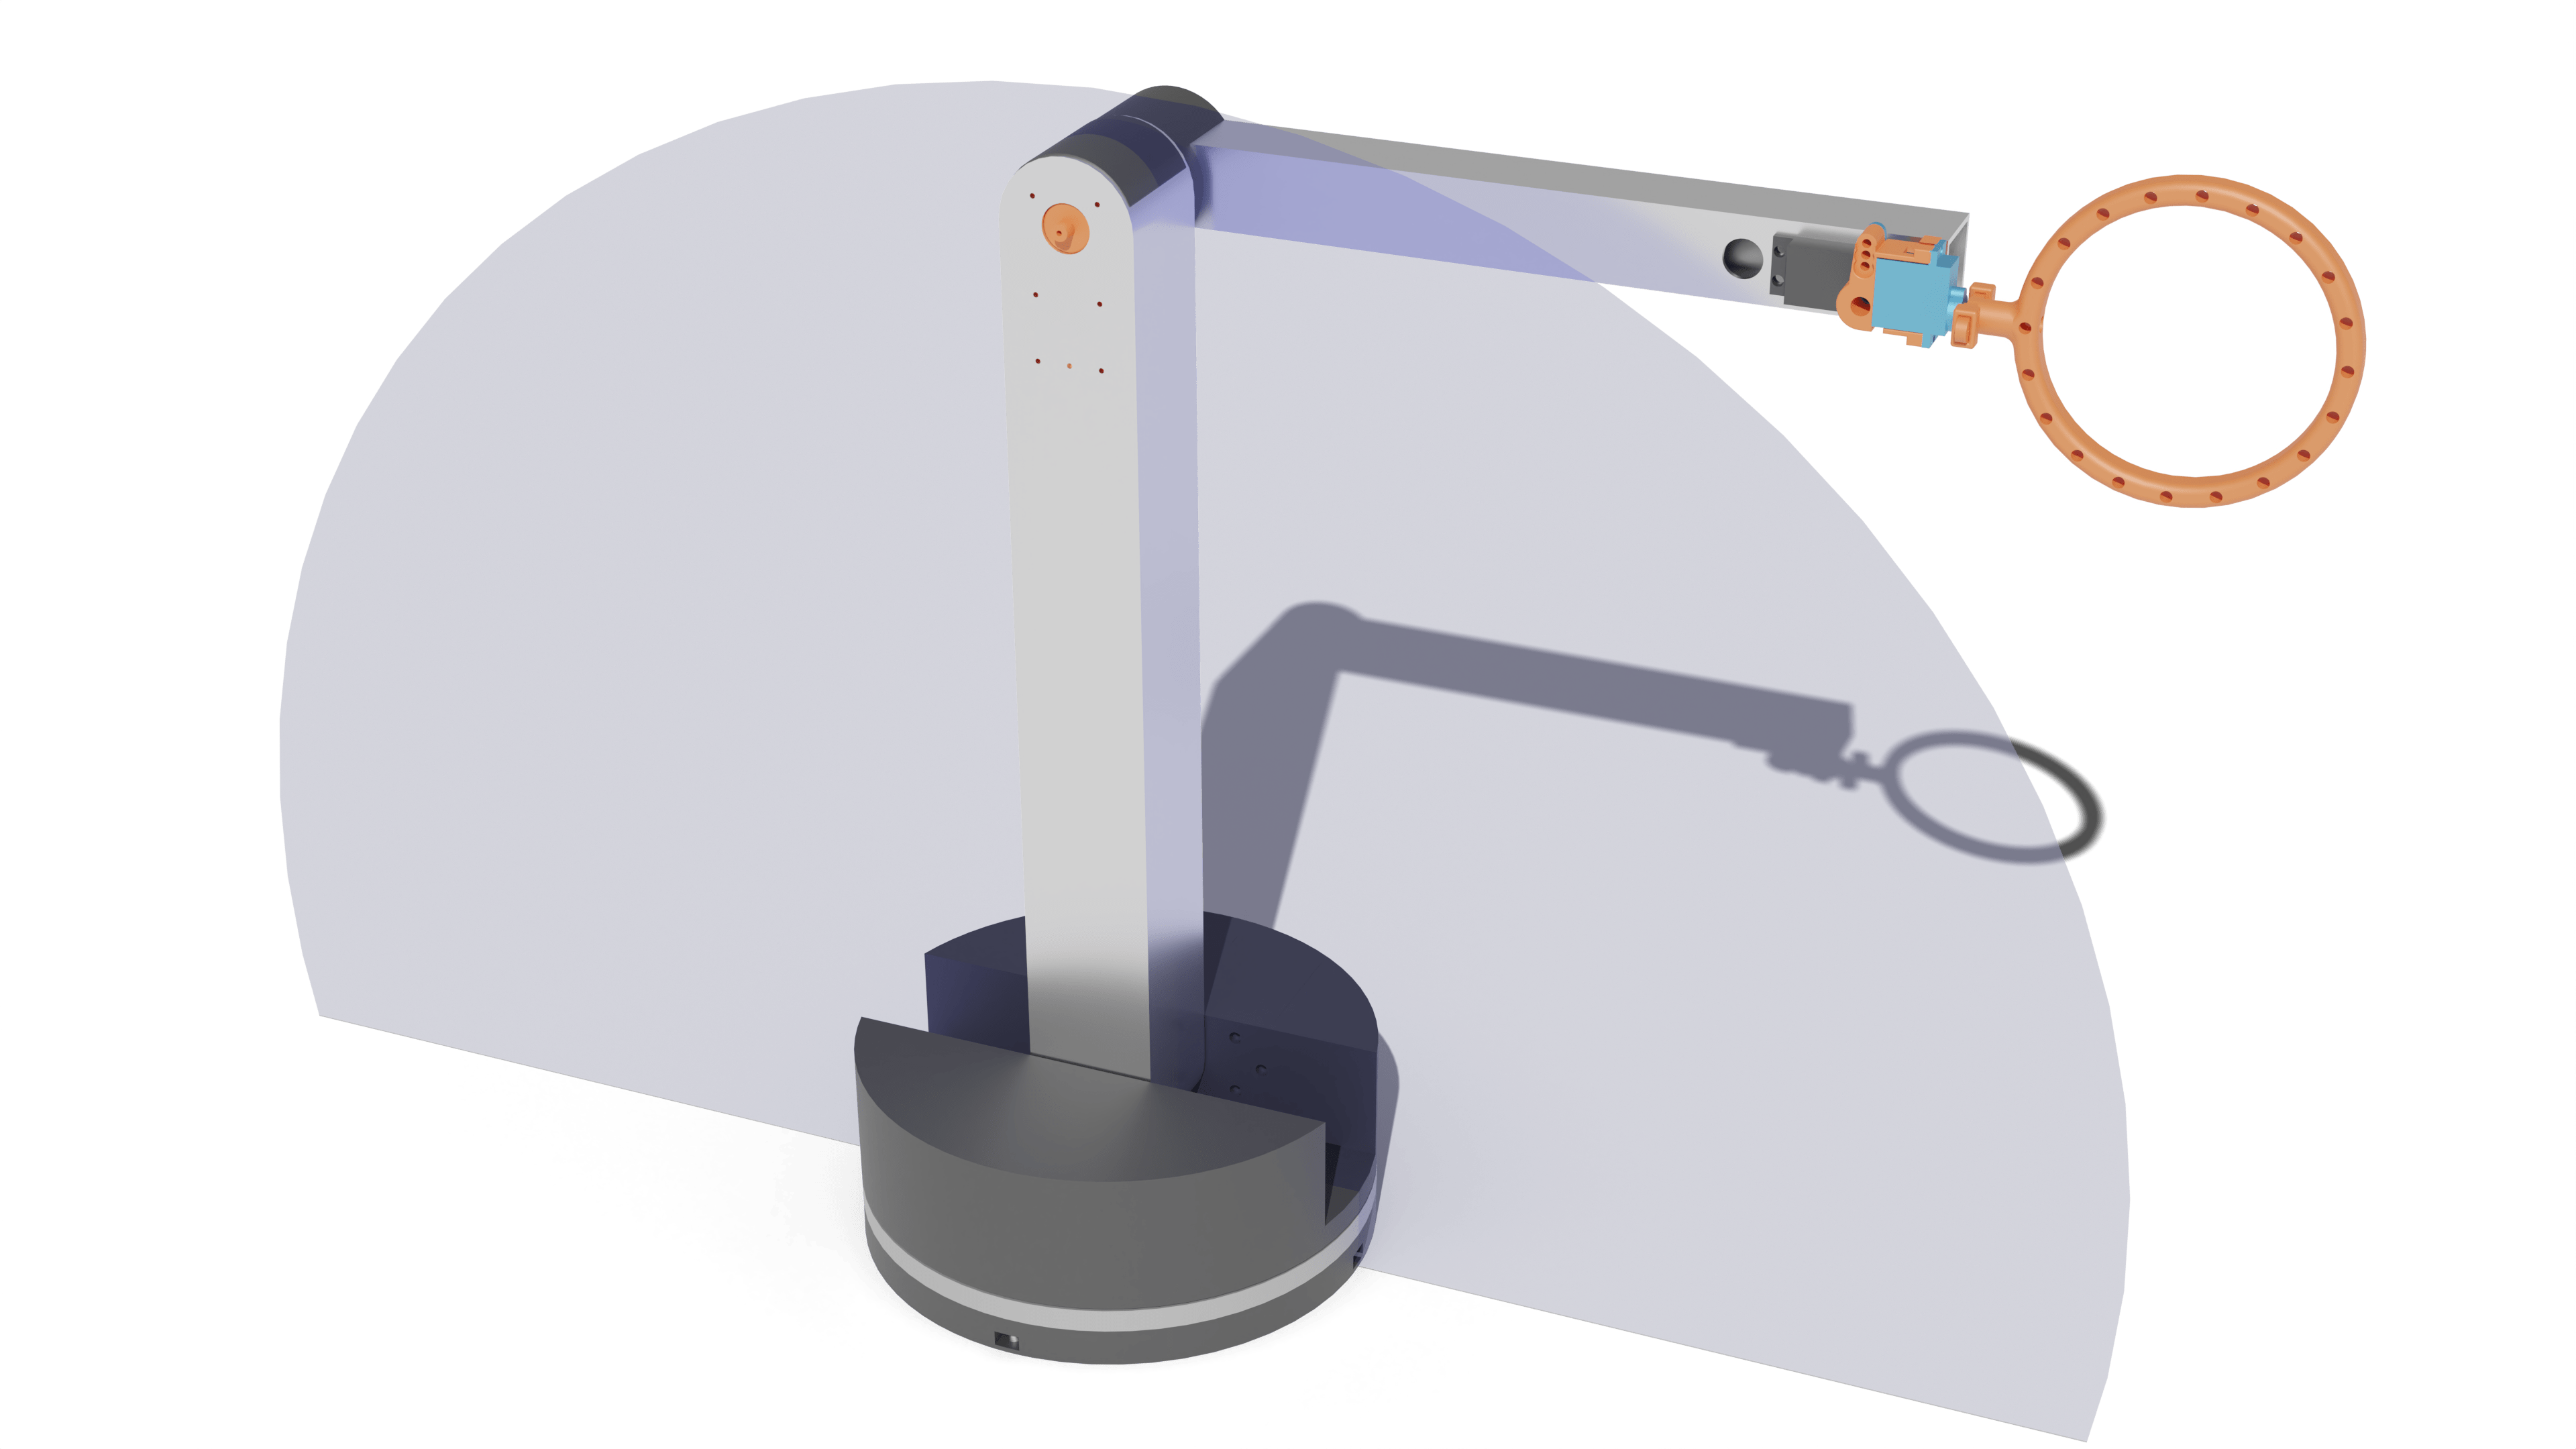
\includegraphics[width=\textwidth]{ArmOnPlane1}
    \end{frame}

    \begin{frame}
        \frametitle{Bauspezifikationen}
        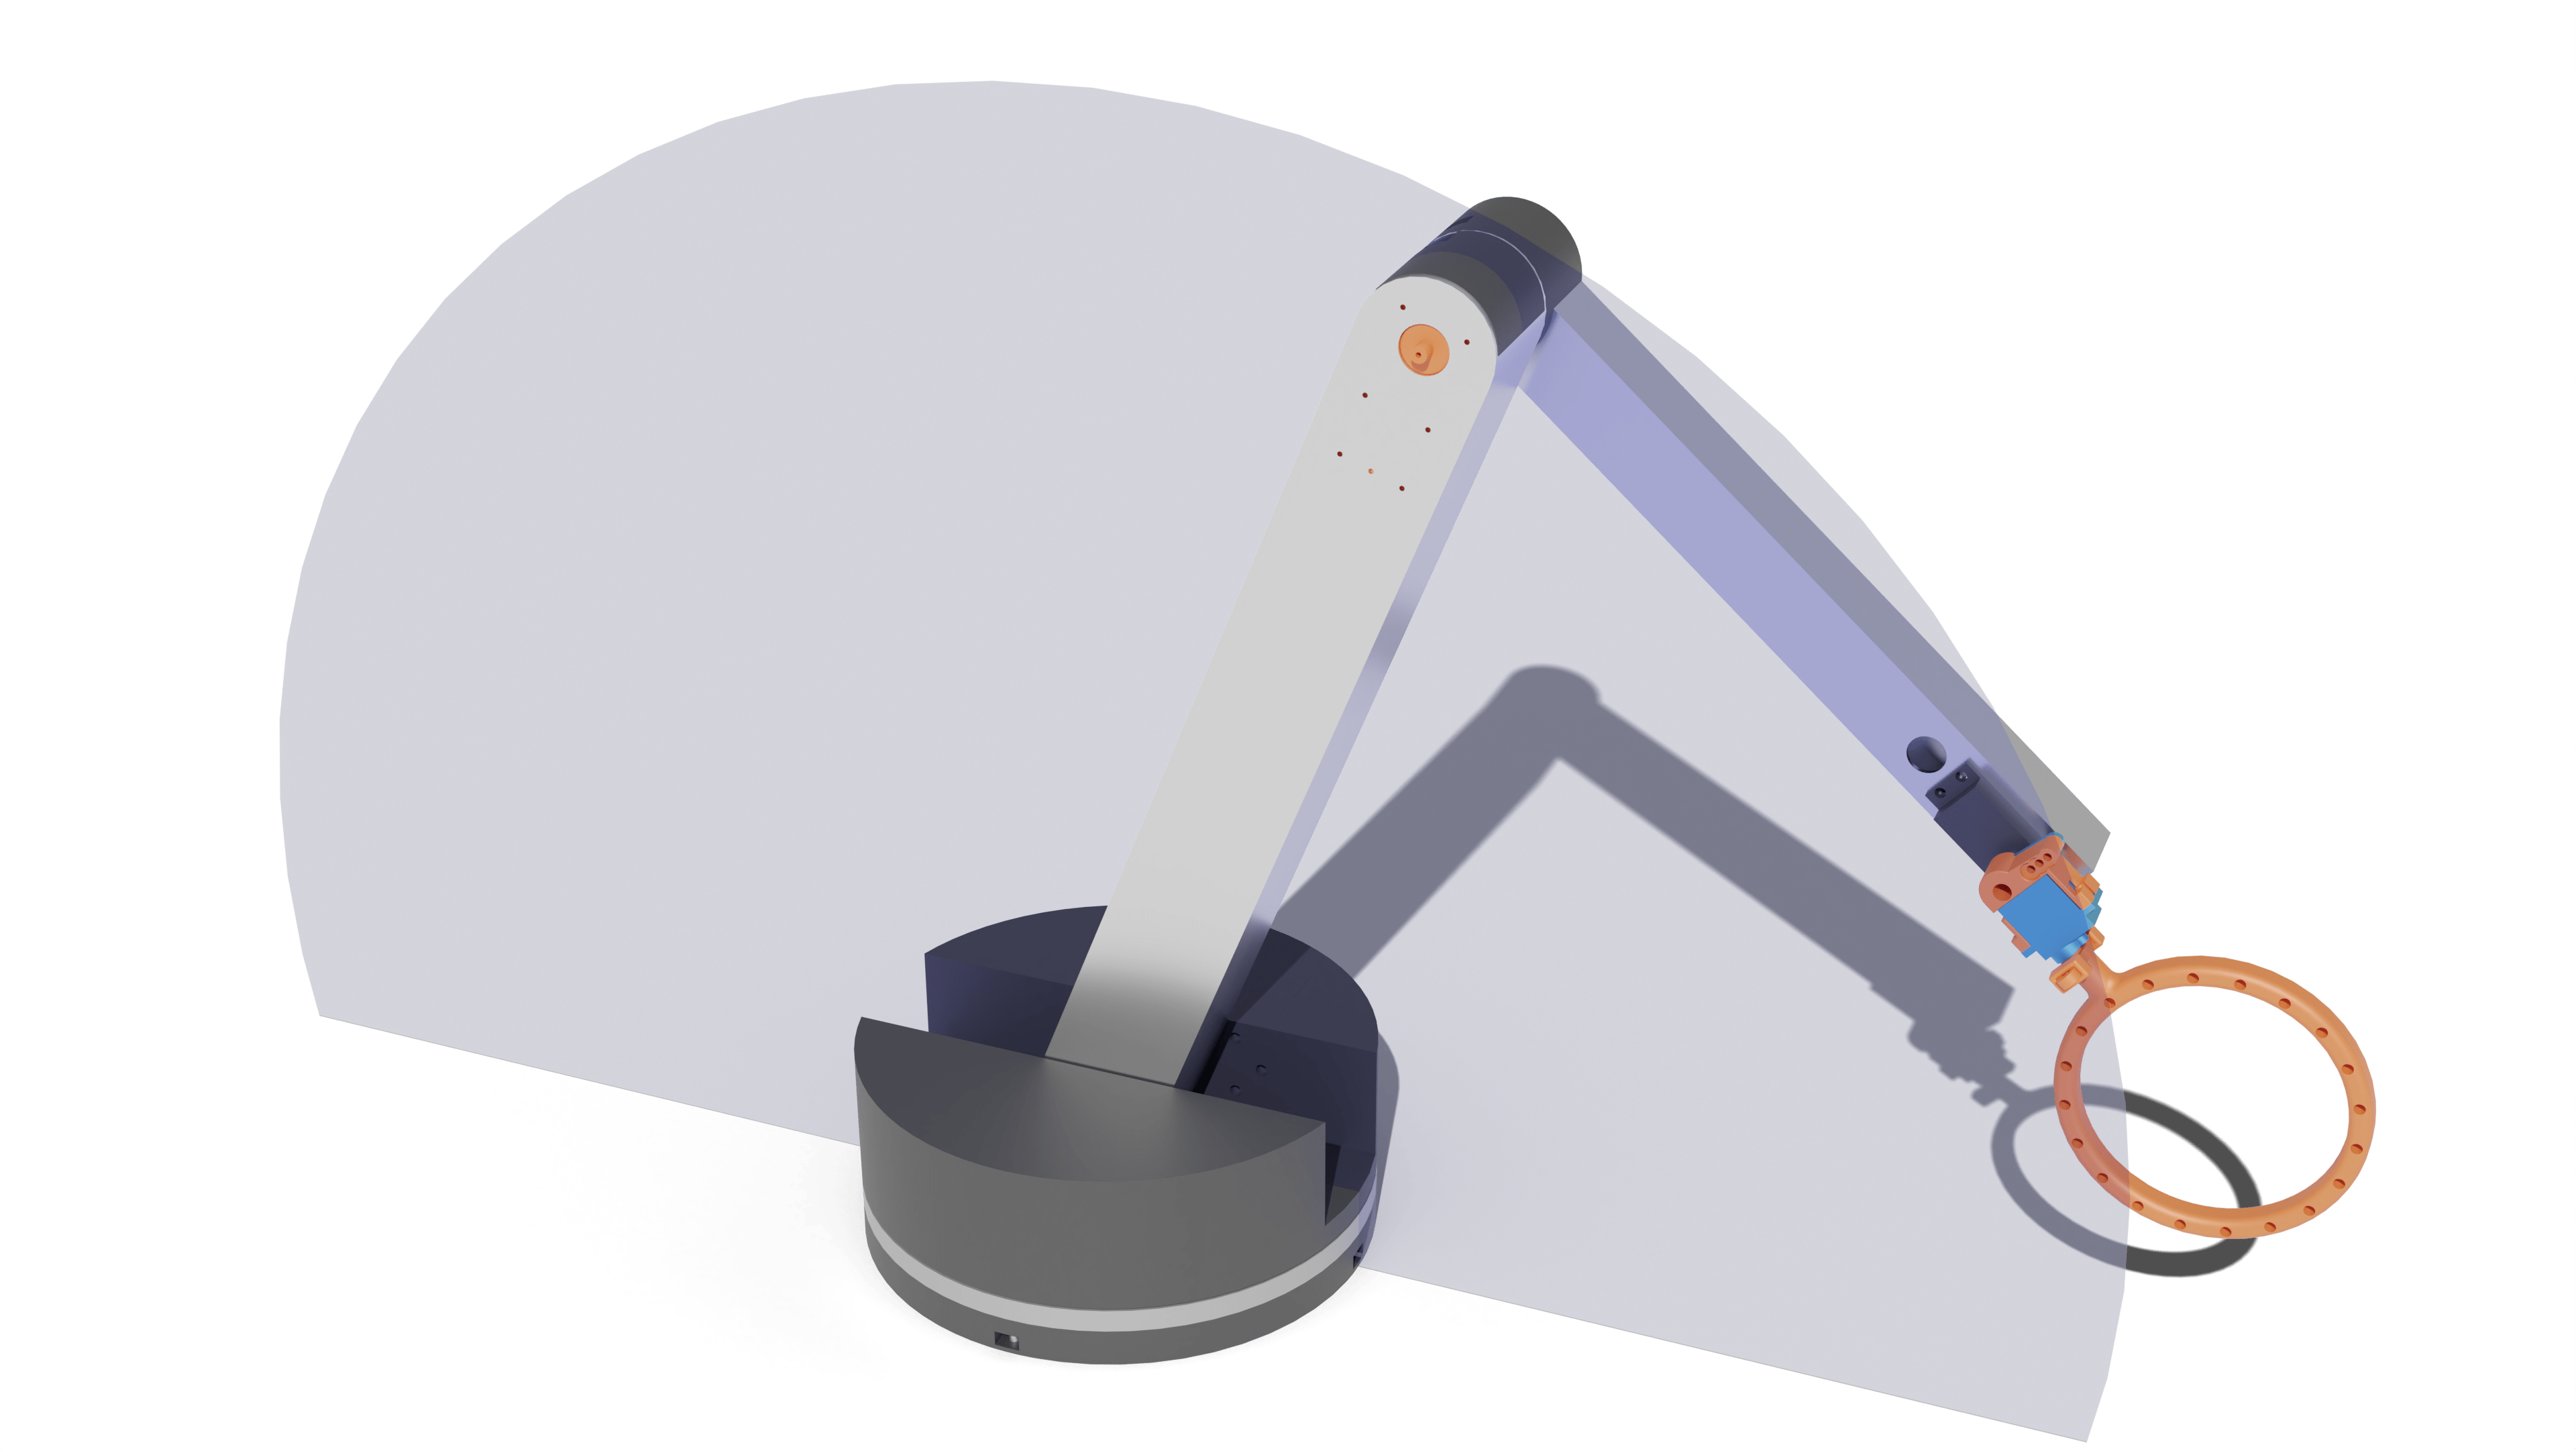
\includegraphics[width=\textwidth]{ArmOnPlane2}
    \end{frame}

    \begin{frame}
        \frametitle{Bauspezifikationen}
        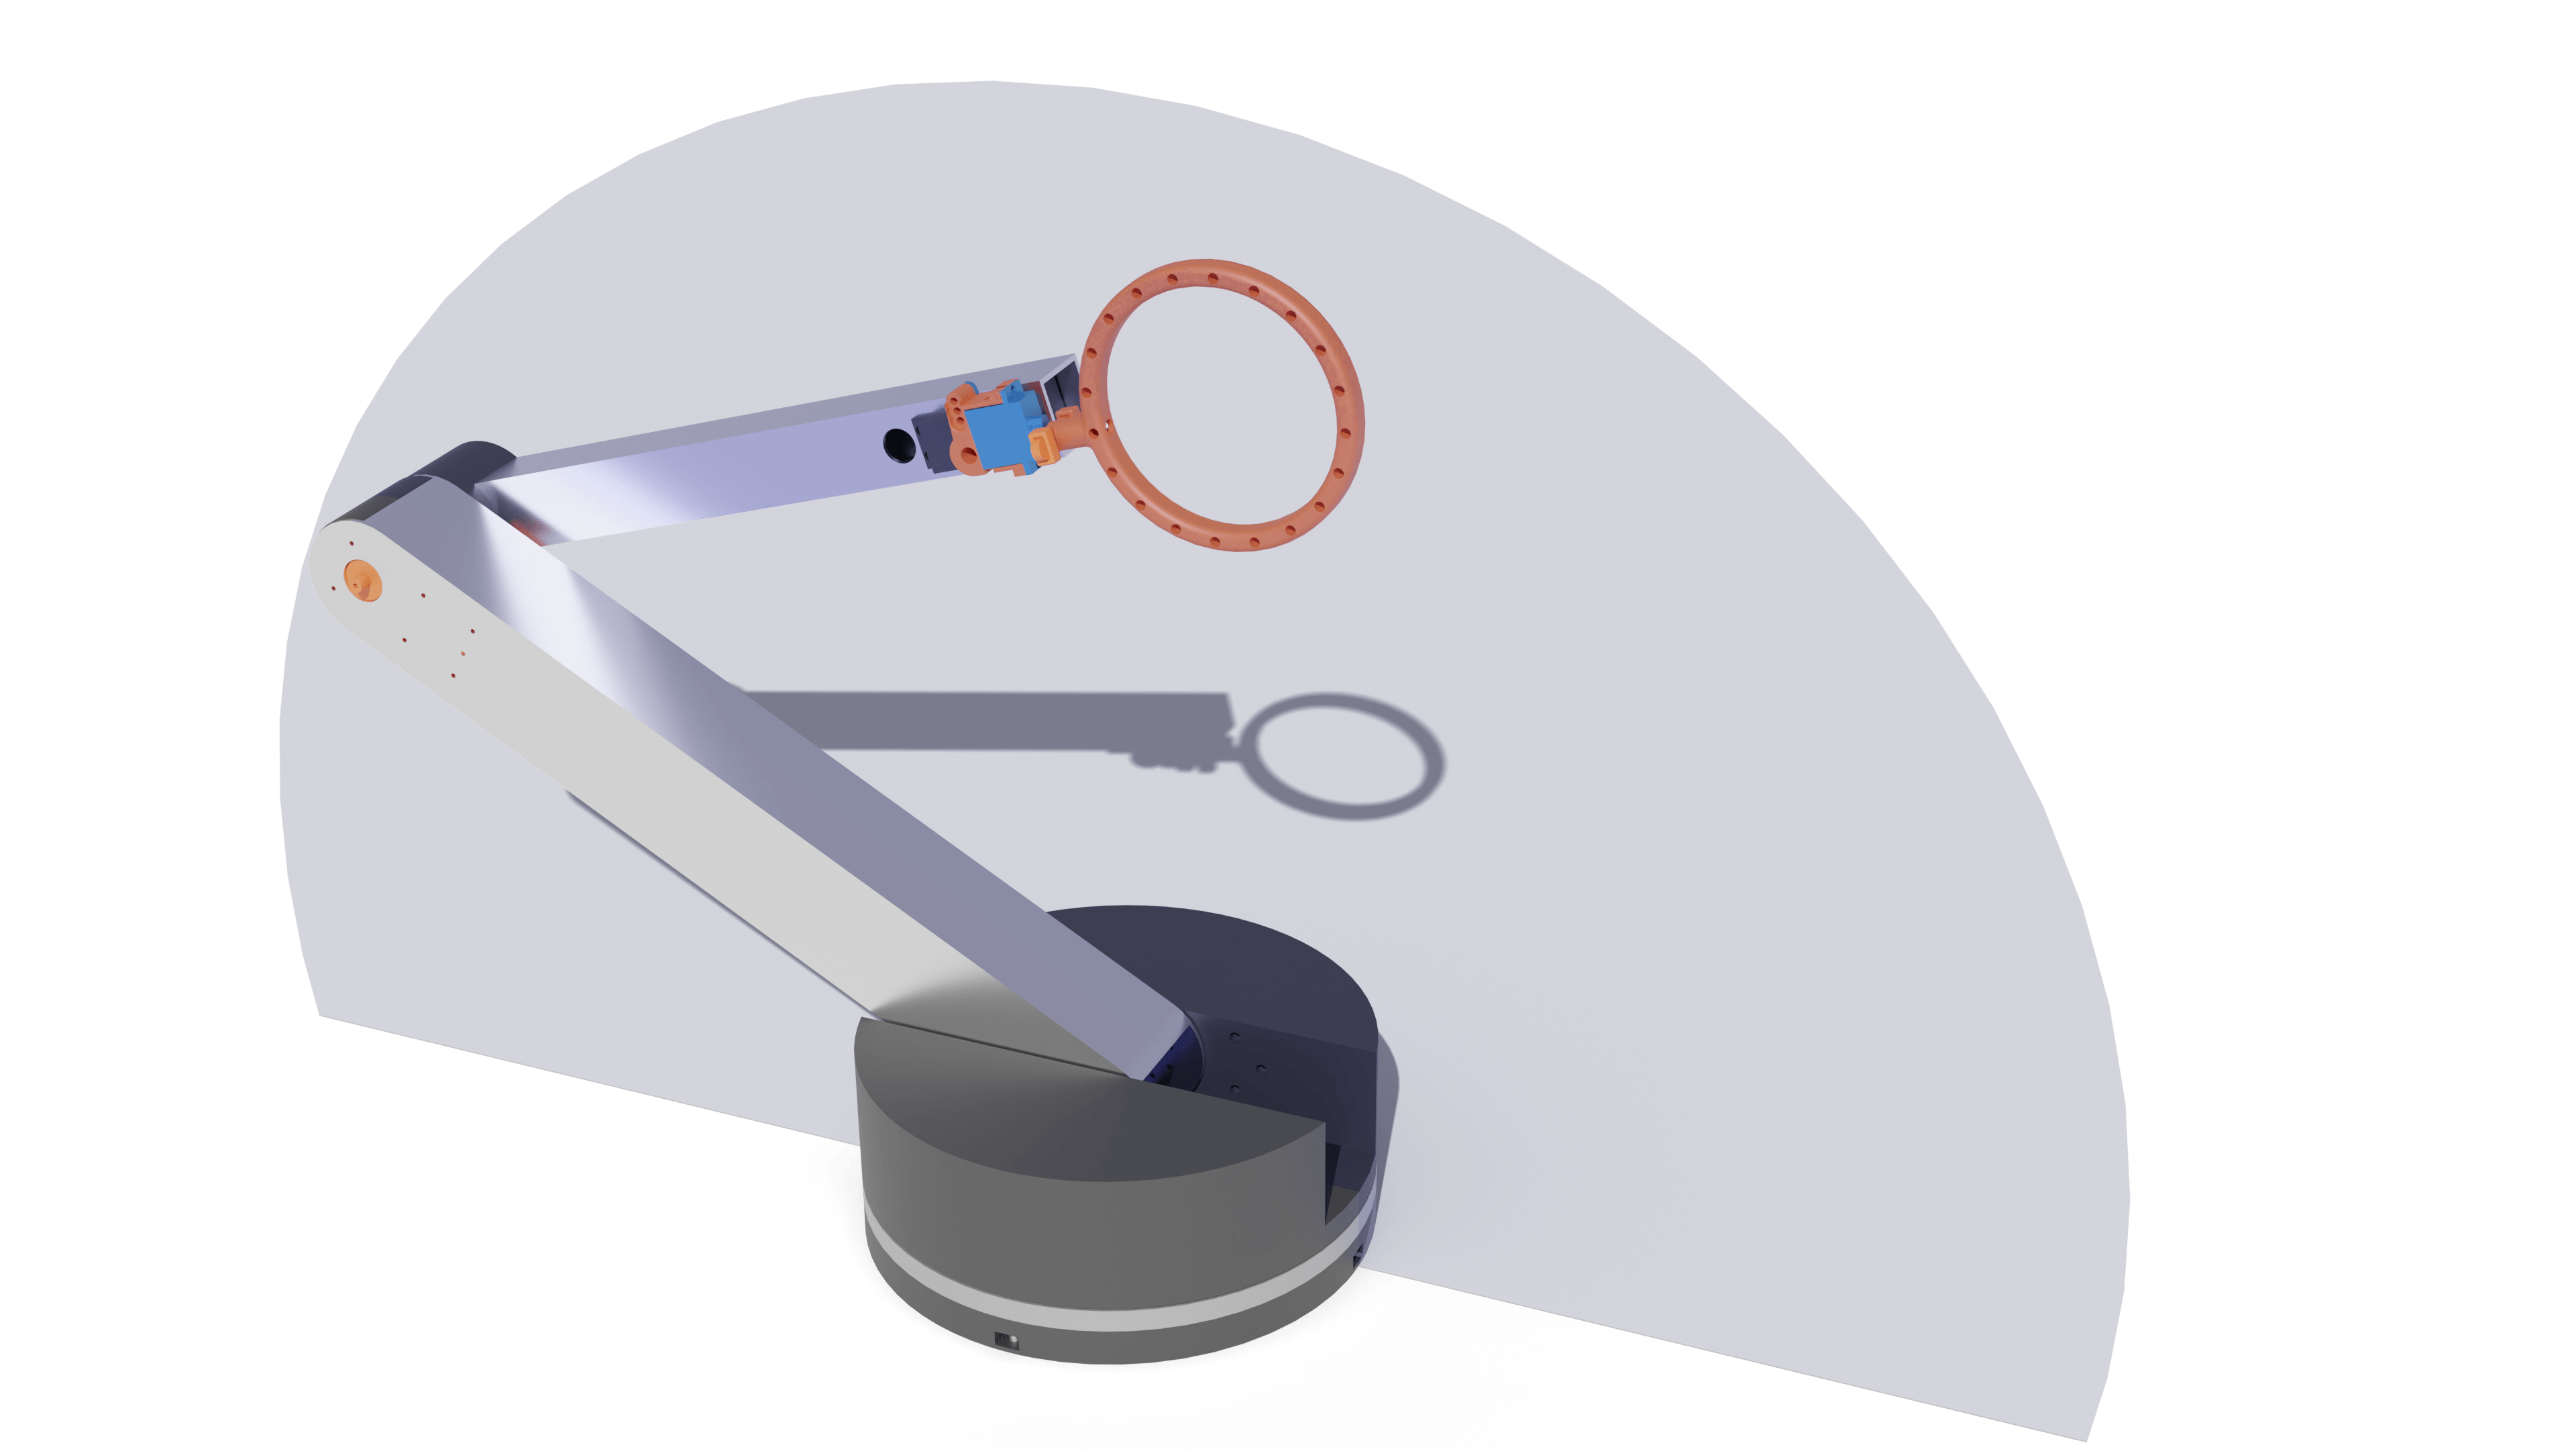
\includegraphics[width=\textwidth]{ArmOnPlane3}
    \end{frame}

    \begin{frame}
        \frametitle{Bauspezifikationen}
        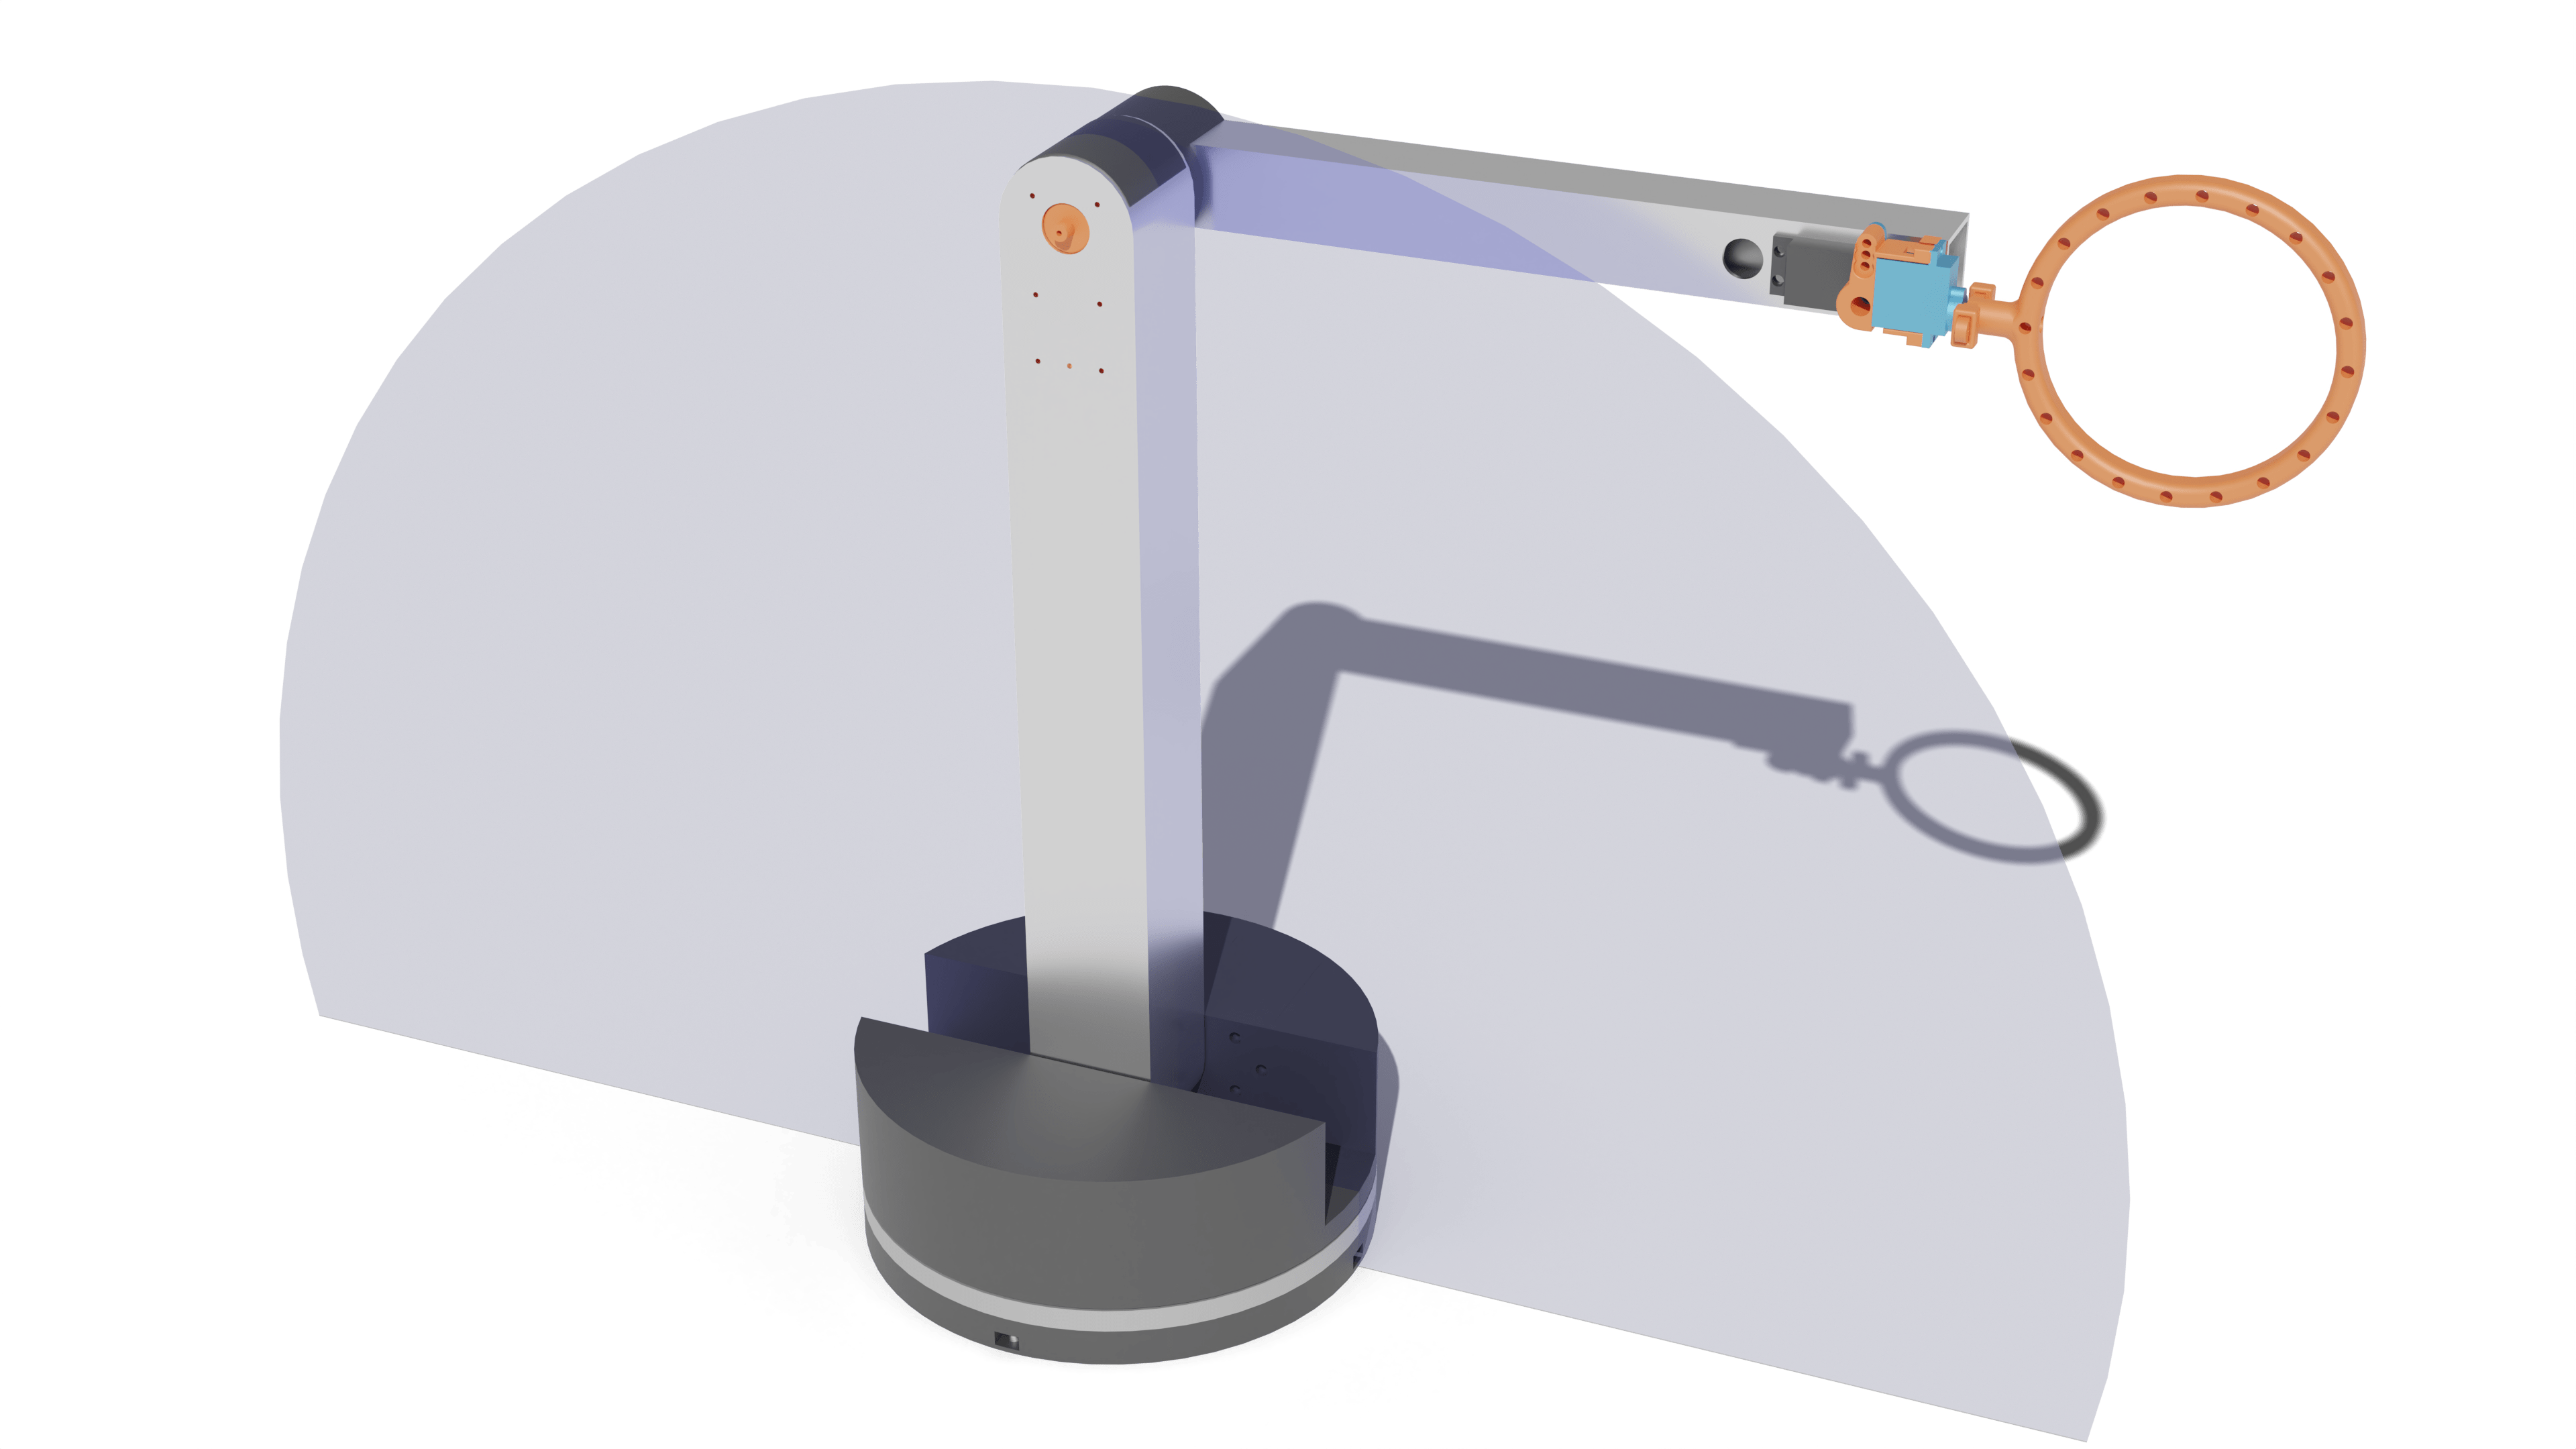
\includegraphics[width=\textwidth]{ArmOnPlane1}
    \end{frame}


\end{document}
